\addcontentsline{toc}{section}{Introduction}

\section*{Introduction}

\section{Définition}
Trino est un moteur de requête SQL distribué open source. Il s'agit d'un hard fork du projet Presto original créé par Facebook. Il permet aux développeurs d'exécuter des analyses interactives sur de gros volumes de données. Avec Trino, les organisations peuvent facilement utiliser leurs compétences SQL existantes pour interroger des données sans avoir à apprendre de nouveaux langages complexes. L'architecture est assez similaire aux systèmes traditionnels de traitement analytique en ligne (OLAP) utilisant des architectures informatiques distribuées, dans lesquelles un nœud de contrôleur coordonne plusieurs nœuds de travail.
\section{Comment ça fonctionne}
Trino est un système distribué qui s'exécute sur Hadoop et utilise une architecture similaire aux bases de données de traitement massivement parallèle (MPP). Il a un nœud coordinateur travaillant avec plusieurs nœuds de travail. Les utilisateurs soumettent SQL au coordinateur qui utilise le moteur de requête et d'exécution pour analyser, planifier et planifier un plan de requête distribué sur les nœuds de travail. Il prend en charge le SQL ANSI standard, y compris les requêtes complexes, les agrégations de jointures et les jointures externes.

Tirant parti de cette architecture, le moteur de requête Trino est capable de traiter des requêtes SQL sur de grandes quantités de données en parallèle sur un cluster d'ordinateurs ou de nœuds. Trino s'exécute en tant que processus à serveur unique sur chaque nœud. Plusieurs nœuds exécutant Trino, qui sont configurés pour collaborer les uns avec les autres, constituent un cluster Trino.

La figure suivante affiche une vue d'ensemble de haut niveau d'un cluster Trino composé d'un coordinateur et de plusieurs nœuds de travail. Un utilisateur Trino se connecte au coordinateur avec un client, tel qu'un outil utilisant le pilote JDBC ou la CLI Trino. Le coordinateur collabore ensuite avec les workers, qui accèdent aux sources de données.

\begin{figure}[htbp]
\centering
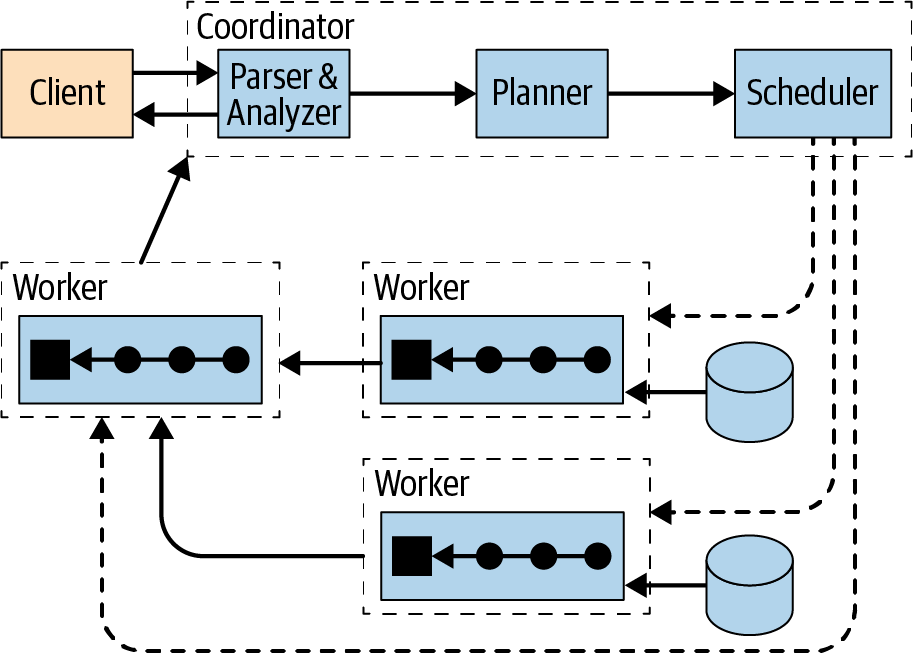
\includegraphics[width=\linewidth]{images/trino_architecture.png}
\caption{Vue d'ensemble de l'architecture Trino avec le coordinateur et les workers}\label{fig:trino-architecture}
\end{figure}

\begin{enumerate}
	\item Un coordinateur est un serveur Trino qui gère les requêtes entrantes et gère les workers pour exécuter les requêtes.
	\item Un worker est un serveur Trino responsable de l'exécution des tâches et du traitement des données.
	\item Le service de découverte s'exécute généralement sur le coordinateur et permet aux workers de s'inscrire pour participer au cluster.
	\item Toutes les communications et tous les transferts de données entre les clients, le coordinateur et les workers utilisent des interactions basées sur REST sur HTTP/HTTPS.
\end{enumerate}

La figure suivante montre comment la communication au sein du cluster se produit entre le coordinateur et les workers, ainsi que d'un worker à l'autre. Le coordinateur discute avec les workers pour attribuer le travail, mettre à jour le statut et récupérer l'ensemble de résultats de niveau supérieur à renvoyer aux utilisateurs. Les workers se parlent pour récupérer des données à partir de tâches en amont, exécutées sur d'autres workers. Et les workers récupèrent les ensembles de résultats à partir de la source de données.

\begin{figure}[htbp]
\centering
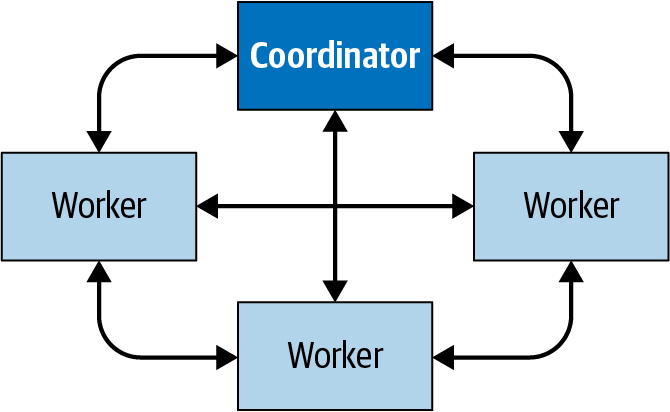
\includegraphics[width=\linewidth]{images/trino_communication.png}
\caption{Communication entre le coordinateur et les workers dans un cluster Trino}\label{fig:trino-communication}
\end{figure}

\section{Coordinateur}
Le coordinateur Trino est le serveur responsable de la réception des instructions SQL des utilisateurs, de l'analyse de ces instructions, de la planification des requêtes et de la gestion des nœuds de travail. C'est le cerveau d'une installation Trino et le nœud auquel un client se connecte. Les utilisateurs interagissent avec le coordinateur via la CLI Trino, les applications utilisant les pilotes JDBC ou ODBC, ou toute autre bibliothèque client disponible pour une variété de langues. Le coordinateur accepte les instructions SQL du client telles que les requêtes SELECT pour l'exécution.

Chaque installation Trino doit avoir un coordinateur aux côtés d'un ou plusieurs workers. À des fins de développement ou de test, une seule instance de Trino peut être configurée pour remplir les deux rôles.

Le coordinateur suit l'activité de chaque worker et coordonne l'exécution d'une requête. Le coordinateur crée un modèle logique d'une requête impliquant une série d'étapes.

Une fois qu'il reçoit une instruction SQL, le coordinateur est responsable de l'analyse, de l'analyse, de la planification et de la planification de l'exécution de la requête sur les nœuds de travail Trino. L'instruction est traduite en une série de tâches connectées s'exécutant sur un cluster de workers. Au fur et à mesure que les workers traitent les données, les résultats sont récupérés par le coordinateur et exposés aux clients sur un tampon de sortie. Une fois qu'un tampon de sortie est complètement lu par le client, le coordinateur demande plus de données aux workers au nom du client. Les workers, à leur tour, interagissent avec les sources de données pour en obtenir les données. En conséquence, les données sont continuellement demandées par le client et fournies par les workers à partir de la source de données jusqu'à ce que l'exécution de la requête soit terminée.

Les coordinateurs communiquent avec les workers et les clients à l'aide d'un protocole basé sur HTTP.
\begin{figure}[htbp]
\centering
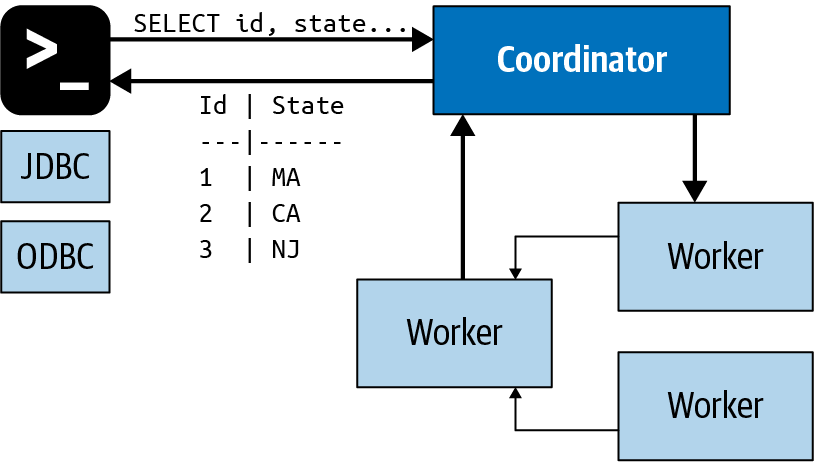
\includegraphics[width=\linewidth]{images/trino_communication_processing.png}
\caption{Communication client, coordinateur et worker traitant une instruction SQL}\label{fig:trino-communication-precessing}
\end{figure}

\section{Workers}
Un worker Trino est un serveur dans une installation Trino. Il est responsable de l'exécution des tâches assignées par le coordinateur et du traitement des données. Les nœuds de travail récupèrent des données à partir de sources de données à l'aide de connecteurs, puis échangent des données intermédiaires entre eux. Les données finales qui en résultent sont transmises au coordinateur. Le coordonnateur est chargé de recueillir les résultats des workers et de fournir les résultats finaux au client.

Lors de l'installation, les agents sont configurés pour connaître le nom d'hôte ou l'adresse IP du service de découverte du cluster. Lorsqu'un agent démarre, il s'annonce au service de découverte, qui le met à la disposition du coordinateur pour l'exécution de la tâche.

Les workers communiquent avec d'autres workers et le coordinateur à l'aide d'un protocole basé sur HTTP.

La figure suivante montre comment plusieurs workers récupèrent des données à partir des sources de données et collaborent pour traiter les données, jusqu'à ce qu'un worker puisse fournir les données au coordinateur.

\begin{figure}[htbp]
\centering
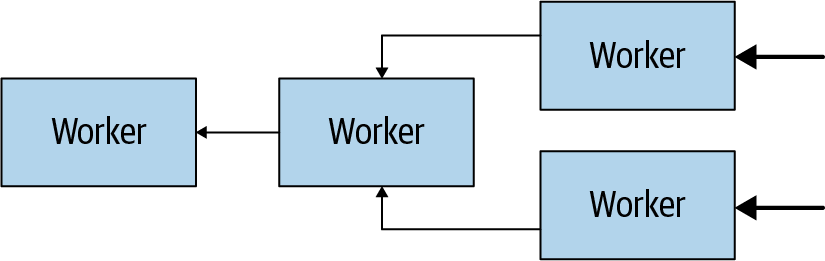
\includegraphics[width=\linewidth]{images/trino_workers.png}
\caption{Les workers d'un cluster collaborent pour traiter les instructions et les données SQL}\label{fig:trino-workers}
\end{figure}

\section{Architecture basée sur les connecteurs}
Au cœur de la séparation du stockage et du calcul dans Trino se trouve l'architecture basée sur les connecteurs. Un connecteur fournit à Trino une interface pour accéder à une source de données arbitraire.

Chaque connecteur fournit une abstraction basée sur une table sur la source de données sous-jacente. Tant que les données peuvent être exprimées en termes de tables, de colonnes et de lignes à l'aide des types de données disponibles pour Trino, un connecteur peut être créé et le moteur de requête peut utiliser les données pour le traitement des requêtes.

Trino fournit une interface de fournisseur de services (SPI), qui est un type d'API utilisé pour implémenter un connecteur. En implémentant le SPI dans un connecteur, Trino peut utiliser des opérations standard en interne pour se connecter à n'importe quelle source de données et effectuer des opérations sur n'importe quelle source de données. Le connecteur prend en charge les détails relatifs à la source de données spécifique.

\begin{enumerate}
	\item[$\bullet$] Opérations pour récupérer les métadonnées de table/vue/schéma
	\item[$\bullet$] Opérations pour produire des unités logiques de partitionnement de données, afin que Trino puisse paralléliser les lectures et les écritures
	\item[$\bullet$] Sources et récepteurs de données qui convertissent les données source vers/depuis le format en mémoire attendu par le moteur de requête 
\end{enumerate}

Trino fournit de nombreux connecteurs aux systèmes, vous trouverez la liste des connecteurs au moment de la rédaction de ce rapport ci-dessous.

% chktex-file 44
\begin{table}[ht]
\centering
	\begin{tabular}{|c|c|}
	\hline
	\textbf{Nom de connecteur} & \textbf{Lien de documentation} \\ \hline
	Accumulo & \href{https://trino.io/docs/current/connector/accumulo.html}{https://trino.io/docs/current/connector/accumulo.html} \\ \hline
	Atop & \href{https://trino.io/docs/current/connector/atop.html}{https://trino.io/docs/current/connector/atop.html} \\ \hline
	BigQuery & \href{https://trino.io/docs/current/connector/bigquery.html}{https://trino.io/docs/current/connector/bigquery.html} \\ \hline
	Black Hole & \href{https://trino.io/docs/current/connector/blackhole.html}{https://trino.io/docs/current/connector/blackhole.html} \\ \hline
	Cassandra & \href{https://trino.io/docs/current/connector/cassandra.html}{https://trino.io/docs/current/connector/cassandra.html} \\ \hline
	ClickHouse & \href{https://trino.io/docs/current/connector/clickhouse.html}{https://trino.io/docs/current/connector/clickhouse.html} \\ \hline
	Delta Lake & \href{https://trino.io/docs/current/connector/delta-lake.html}{https://trino.io/docs/current/connector/delta-lake.html} \\ \hline
	Druid & \href{https://trino.io/docs/current/connector/druid.html}{https://trino.io/docs/current/connector/druid.html} \\ \hline
	Elasticsearch & \href{https://trino.io/docs/current/connector/elasticsearch.html}{https://trino.io/docs/current/connector/elasticsearch.html} \\ \hline
	Google Sheets & \href{https://trino.io/docs/current/connector/googlesheets.html}{https://trino.io/docs/current/connector/googlesheets.html} \\ \hline
	Hive & \href{https://trino.io/docs/current/connector/hive.html}{https://trino.io/docs/current/connector/hive.html} \\ \hline
	Hudi & \href{https://trino.io/docs/current/connector/hudi.html}{https://trino.io/docs/current/connector/hudi.html} \\ \hline
	Iceberg & \href{https://trino.io/docs/current/connector/iceberg.html}{https://trino.io/docs/current/connector/iceberg.html} \\ \hline
	Ignite & \href{https://trino.io/docs/current/connector/ignite.html}{https://trino.io/docs/current/connector/ignite.html} \\ \hline
	JMX & \href{https://trino.io/docs/current/connector/jmx.html}{https://trino.io/docs/current/connector/jmx.html} \\ \hline
	Kafka & \href{https://trino.io/docs/current/connector/kafka.html}{https://trino.io/docs/current/connector/kafka.html} \\ \hline
	Kinesis & \href{https://trino.io/docs/current/connector/kinesis.html}{https://trino.io/docs/current/connector/kinesis.html} \\ \hline
	Kudu & \href{https://trino.io/docs/current/connector/kudu.html}{https://trino.io/docs/current/connector/kudu.html} \\ \hline
	Local File & \href{https://trino.io/docs/current/connector/localfile.html}{https://trino.io/docs/current/connector/localfile.html} \\ \hline
	MariaDB & \href{https://trino.io/docs/current/connector/mariadb.html}{https://trino.io/docs/current/connector/mariadb.html} \\ \hline
	Memory & \href{https://trino.io/docs/current/connector/memory.html}{https://trino.io/docs/current/connector/memory.html} \\ \hline
	MongoDB & \href{https://trino.io/docs/current/connector/mongodb.html}{https://trino.io/docs/current/connector/mongodb.html} \\ \hline
	MySQL & \href{https://trino.io/docs/current/connector/mysql.html}{https://trino.io/docs/current/connector/mysql.html} \\ \hline
	Oracle & \href{https://trino.io/docs/current/connector/oracle.html}{https://trino.io/docs/current/connector/oracle.html} \\ \hline
	Phoenix & \href{https://trino.io/docs/current/connector/phoenix.html}{https://trino.io/docs/current/connector/phoenix.html} \\ \hline
	Pinot & \href{https://trino.io/docs/current/connector/pinot.html}{https://trino.io/docs/current/connector/pinot.html} \\ \hline
	PostgreSQL & \href{https://trino.io/docs/current/connector/postgresql.html}{https://trino.io/docs/current/connector/postgresql.html} \\ \hline
	Prometheus & \href{https://trino.io/docs/current/connector/prometheus.html}{https://trino.io/docs/current/connector/prometheus.html} \\ \hline
	Redis & \href{https://trino.io/docs/current/connector/redis.html}{https://trino.io/docs/current/connector/redis.html} \\ \hline
	Redshift & \href{https://trino.io/docs/current/connector/redshift.html}{https://trino.io/docs/current/connector/redshift.html} \\ \hline
	SingleStore & \href{https://trino.io/docs/current/connector/singlestore.html}{https://trino.io/docs/current/connector/singlestore.html} \\ \hline
	SQL Server & \href{https://trino.io/docs/current/connector/sqlserver.html}{https://trino.io/docs/current/connector/sqlserver.html} \\ \hline
	System & \href{https://trino.io/docs/current/connector/system.html}{https://trino.io/docs/current/connector/system.html} \\ \hline
	Thrift & \href{https://trino.io/docs/current/connector/thrift.html}{https://trino.io/docs/current/connector/thrift.html} \\ \hline
	TPCDS & \href{https://trino.io/docs/current/connector/tpcds.html}{https://trino.io/docs/current/connector/tpcds.html} \\ \hline
	TPCH & \href{https://trino.io/docs/current/connector/tpch.html}{https://trino.io/docs/current/connector/tpch.html} \\ \hline
\end{tabular}
\caption{Liste des connecteurs Trino et leur documentation}
\end{table}

Le SPI de Trino vous donne également la possibilité de créer vos propres connecteurs personnalisés. Cela peut être nécessaire si vous avez besoin d'accéder à une source de données sans connecteur compatible. Si vous finissez par créer un connecteur, nous vous encourageons fortement à en savoir plus sur la communauté open source Trino, à utiliser notre aide et à contribuer votre connecteur. Consultez « Ressources Trino » pour plus d'informations. Un connecteur personnalisé peut également être nécessaire si vous disposez d'une source de données unique ou propriétaire au sein de votre organisation. C'est ce qui permet aux utilisateurs de Trino d'interroger n'importe quelle source de données en utilisant SQL, vraiment SQL-on-Anything.

La figure suivante montre comment le Trino SPI inclut des interfaces distinctes pour les métadonnées, les statistiques de données et l'emplacement des données utilisées par le coordinateur, et pour le flux de données utilisé par les workers.

\begin{figure}[htbp]
\centering
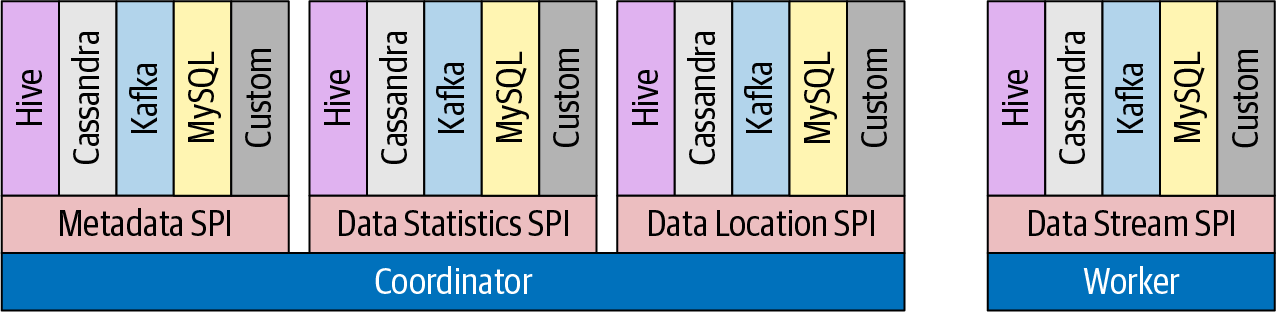
\includegraphics[width=\linewidth]{images/trino_connector.png}
\caption{Vue d'ensemble de l'interface du fournisseur de services Trino (SPI)}\label{fig:trino-connector}
\end{figure}

Les connecteurs Trino sont des plug-ins chargés par chaque serveur au démarrage. Ils sont configurés par des paramètres spécifiques dans les fichiers de propriétés du catalogue et chargés à partir du répertoire des plug-ins.

\section{Catalogues, Schémas et Tables}
Le cluster Trino traite toutes les requêtes en utilisant l'architecture basée sur les connecteurs décrite précédemment. Chaque configuration de catalogue utilise un connecteur pour accéder à une source de données spécifique. La source de données expose un ou plusieurs schémas dans le catalogue. Chaque schéma contient des tables qui fournissent les données dans des lignes de table avec des colonnes utilisant différents types de données. Vous pouvez en savoir plus sur les catalogues, les schémas, les tables. Plus précisément dans `Catalogues', `Schémas' et `Tables'.

\addcontentsline{toc}{section}{Conclusion}
\section*{Conclusion}
L'architecture Trino a un coordinateur recevant les demandes des utilisateurs, puis utilisant des travailleurs pour assembler toutes les données à partir des sources de données. Chaque requête est traduite en un plan de requête distribué de tâches en plusieurs étapes. Les données sont renvoyées par les connecteurs en fractions et traitées en plusieurs étapes jusqu'à ce que le résultat final soit disponible et fourni à l'utilisateur par le coordinateur.